% !TeX spellcheck = en_US
\usetikzlibrary{calc,arrows.meta,positioning}
\tikzset{
    every node/.style={font=\sffamily\small},
    main node/.style={shape=rectangle, rounded corners,
    	draw, align=center,
    	top color=white, bottom color=blue!20}
}

\begin{figure}
	\centering
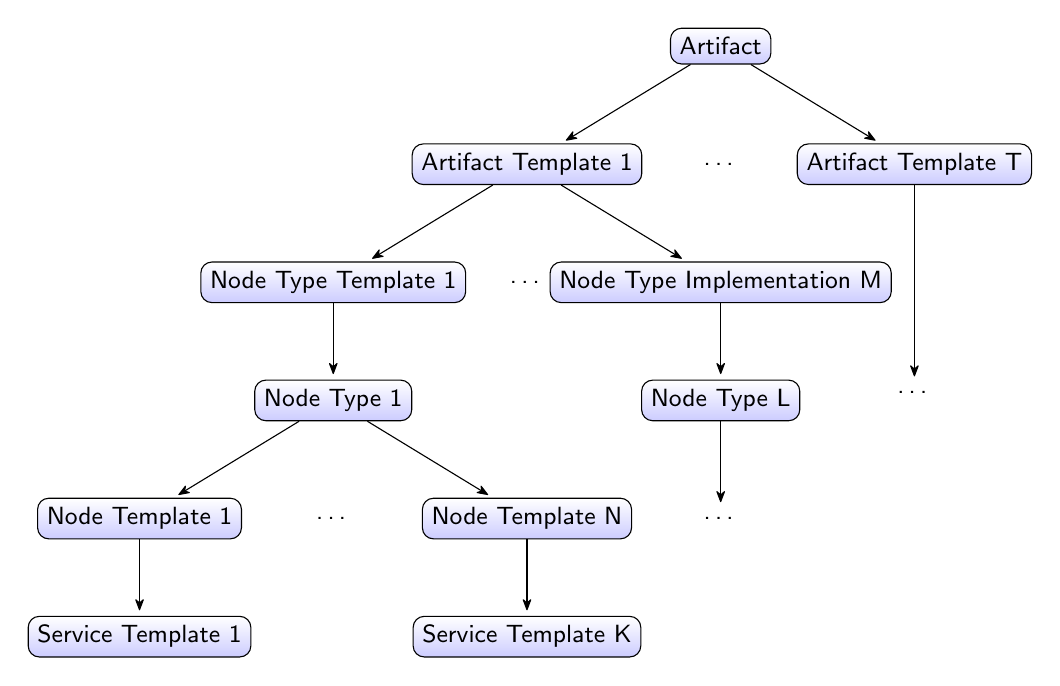
\begin{tikzpicture}[sibling distance=14em,->,>={Stealth[round,sep]},shorten >=1pt,auto,node distance=25mm]
    \node[main node] (1) {Artifact}
    child { node[main node](3) {Artifact Template 1} 
    	child { node[main node] (6) {Node Type Template 1} 
    			child { node[main node] (8) {Node Type 1} 
    				child { node[main node]  (11) {Node Template 1} 
    					child { node[main node] (13) {Service Template 1}}  
    				}
    				child { node[main node]  (12) {Node Template N} 
    					child { node[main node] (14) {Service Template K}}
    				}
    			}
    	}
    	child { node[main node] (7) {Node Type Implementation M} 
    		child { node[main node] (9) {Node Type L} 
    			child { node  (10) {\ldots} }
    		}
    	}
    }
    child { node[main node] (4) {Artifact Template T}  
    child { node (5) [below =of 4]{\ldots}}
	};

    \node at ($(3)!.5!(4)$) {\ldots};
    \node at ($(6)!.5!(7)$) {\ldots};
    \node at ($(11)!.5!(12)$) {\ldots};
    
\end{tikzpicture} 
\caption{An example tree describing how to find Service Templates and Node Templates for the given script} 	\label{fig:script_serv}
\end{figure}